\documentclass[journal]{IEEEtran}
\usepackage[a5paper, margin=10mm]{geometry}
%\usepackage{lmodern} % Ensure lmodern is loaded for pdflatex
\usepackage{tfrupee} % Include tfrupee package


\setlength{\headheight}{1cm} % Set the height of the header box
\setlength{\headsep}{0mm}     % Set the distance between the header box and the top of the text


%\usepackage[a5paper, top=10mm, bottom=10mm, left=10mm, right=10mm]{geometry}

%
\setlength{\intextsep}{10pt} % Space between text and floats

\makeindex


\usepackage{cite}
\usepackage{amsmath,amssymb,amsfonts,amsthm}
\usepackage{algorithmic}
\usepackage{graphicx}
\usepackage{textcomp}
\usepackage{xcolor}
\usepackage{txfonts}
\usepackage{listings}
\usepackage{enumitem}
\usepackage{mathtools}
\usepackage{gensymb}
\usepackage{comment}
\usepackage[breaklinks=true]{hyperref}
\usepackage{tkz-euclide} 
\usepackage{listings}
\usepackage{multicol}
\usepackage{xparse}
\usepackage{gvv}
%\def\inputGnumericTable{}                                 
\usepackage[latin1]{inputenc}                                
\usepackage{color}                                            
\usepackage{array}                                            
\usepackage{longtable}                                       
\usepackage{calc}                                             
\usepackage{multirow}                                         
\usepackage{hhline}                                           
\usepackage{ifthen}                                               
\usepackage{lscape}
\usepackage{tabularx}
\usepackage{array}
\usepackage{float}
\usepackage{ar}
\usepackage[version=4]{mhchem}


\newtheorem{theorem}{Theorem}[section]
\newtheorem{problem}{Problem}
\newtheorem{proposition}{Proposition}[section]
\newtheorem{lemma}{Lemma}[section]
\newtheorem{corollary}[theorem]{Corollary}
\newtheorem{example}{Example}[section]
\newtheorem{definition}[problem]{Definition}
\newcommand{\BEQA}{\begin{eqnarray}}
\newcommand{\EEQA}{\end{eqnarray}}

\theoremstyle{remark}


\begin{document}
\bibliographystyle{IEEEtran}
\onecolumn

\title{5.13.53}
\author{INDHIRESH S- EE25BTECH11027}
\maketitle


\renewcommand{\thefigure}{\theenumi}
\renewcommand{\thetable}{\theenumi}

\textbf{Question} Given
\begin{align*}
    2x - y + 2z = 2\\
    x - 2y + z = -4\\
    x + y + \lambda z = 4
\end{align*}
then the value of $\lambda$ such that the given system of equation has NO solution, is
\begin{enumerate}
    \item 3
    \item 1
    \item 0
    \item -3
\end{enumerate}
\textbf{Solution}:\\
Let us solve the given equation theoretically and then verify the solution computationally. \\
The given equation can be combined as:
\begin{align}
    \Vec{A}\Vec{x}=\Vec{C}
\end{align}
\begin{align}
  \myvec{2&-1&2\\1&-2&1\\1&1&\lambda}\Vec{x}=\myvec{2\\-4\\4}
\end{align}
Where,
\begin{align}
   \Vec{A}=\myvec{2&-1&2\\1&-2&1\\1&1&\lambda}\;\;and\;\;\Vec{C}=\myvec{2\\-4\\4}
\end{align}
Now forming the augmented matrix:
\begin{align}
[\Vec{A}|\Vec{C}]=  \augvec{3}{1}{2&-1&2&2\\1&-2&1&-4\\1&1&\lambda &4}
\end{align}

\begin{align}
  \augvec{3}{1}{2&-1&2&2\\1&-2&1&-4\\1&1&\lambda &4}\xleftrightarrow[R_1\longleftarrow R_1-2R_2]{R_3\longleftarrow R_3-R_2}  \augvec{3}{1}{0 & 3 & 0&10\\1 & -2 & 1&-4\\1 & 1& \lambda&4}
\end{align}

\begin{align}
      \augvec{3}{1}{0 & 3 & 0&10\\1 & -2 & 1&-4\\1 & 1& \lambda&4}\xleftrightarrow{R_3\longleftarrow R_3-R_2}  \augvec{3}{1}{0 & 3 & 0&10\\1 & -2 & 1&-4\\ 0& 3& \lambda -1&8}
\end{align}

\begin{align}
    \augvec{3}{1}{0 & 3 & 0&10\\1 & -2 & 1&-4\\ 0& 3& \lambda -1&8} \xleftrightarrow{R_3\longleftarrow R_3-R_1} \augvec{3}{1}{0 & 3 & 0&10\\1 & -2 & 1&-4\\ 0& 0& \lambda -1&-2}
\end{align}
Given that the system of equation has NO solution . So,
\begin{align}
    \lambda=1
\end{align}


From the figure it is clearly verified that the theoretical solution matches with the computational solution.\\
\begin{figure}[h]
    \centering
    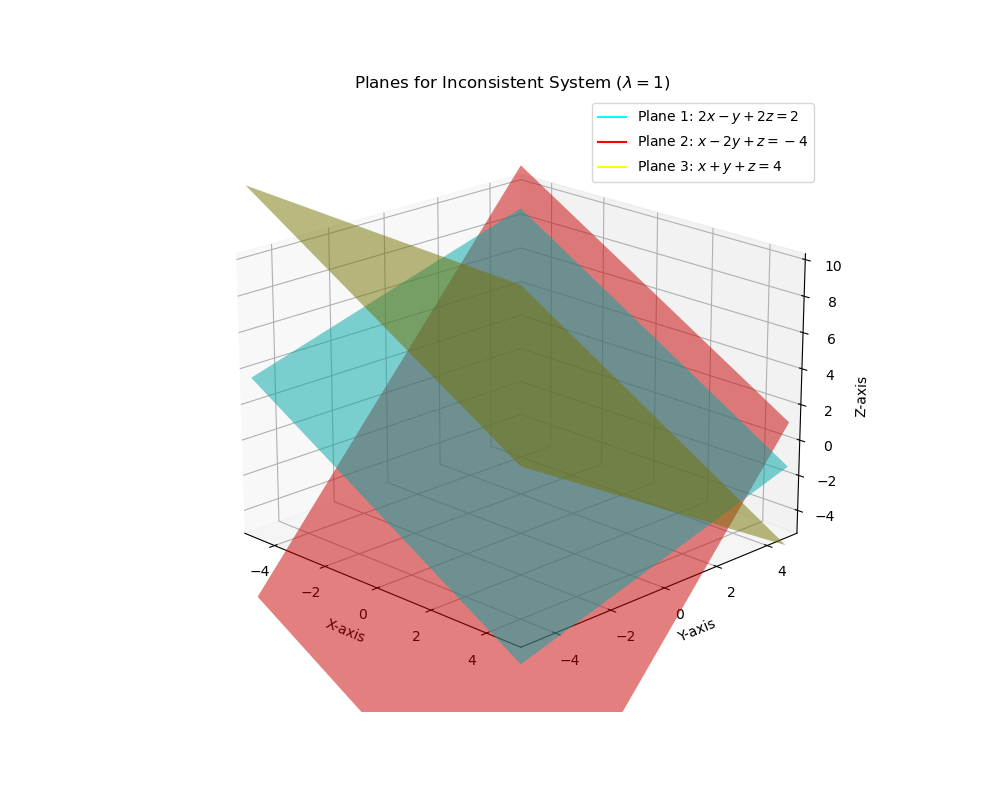
\includegraphics[height=0.5\textheight, keepaspectratio]{figs/figure1.png}
    \label{figure_1}
\end{figure}

\end{document}